\chapter{Marco teórico}
\label{chap:marco-teorico}
\begin{figure}[H]
\centering
\includegraphics[width=0.8\textwidth]{figuras/ProcedimientoCalculoRadiacionInclinada.pdf}
\caption{\label{fig:orge9b78b1}El procedimiento de cálculo consiste en obtener la irradiancia efectiva a partir de la irradiación global en un plano horizontal. Primero, se separan las componentes directa y difusa utilizando índices de claridad y fracciones difusas. Luego, se trasladan estos valores al plano inclinado y se ajustan por factores de suciedad y sombras. Con la irradiancia efectiva y la eficiencia del sistema fotovoltaico, se calcula la potencia en corriente continua, que luego se convierte en corriente alterna a través de un inversor. Finalmente, al integrar esta potencia, se obtiene la energía. Figura modificada de la figura 3.3 del libro ESF \cite{Perpinan2023}.}
\end{figure}


El paquete \texttt{solaR2} toma como marco teórico el libro de Oscar Perpiñán, tutor de este trabajo, Energía Solar Fotovoltaica \cite{Perpinan2023} para cada una de las operaciones de cálculo que realizan cada una de las funciones.
En la figura \ref{fig:orge9b78b1}, se muestra un diagrama que resume los pasos que se siguen a la hora de calcular la producción de sistemas fotovoltaicos.

\FloatBarrier

Estos pasos son:
\begin{enumerate}
\item Calcular la geometría que define la posición relativa del Sol desde la Tierra.
\item Obtener la irradiación global diaria en el plano horizontal.
\item A partir de la irradiación global, obtener las componentes de difusa y directa.
\item Trasladar estos valores de irradiación a valores de irradiancia.
\item Integrando estos valores, obtener las estimaciones irradiación diaria difusa, directa y global.
\item El generador fotovoltaico produce una potencia en corriente continua dependiente del rendimiento del mismo.
\item Un inversor, el cual tiene una efciencia asociada, convierte esta potencia en corriente alterna.
\item Integrar esta potencia para obtener la energía que produce el generador en un tiempo determinado.
\end{enumerate}


\section{Radiación solar}
\label{sec:orge5c8683}
\label{radiacion-solar}
\subsection{Geometría Sol y Tierra}
\label{sec:orgefe3885}
Como es sabido, el movimiento terrestre se compone de una traslación alrededor del Sol y un giro sobre su eje. En este movimiento, la Tierra se desplaza alrededor del Sol siguiendo una elipse de baja excentricidad en la que el Sol ocupa uno de los focos. La duración de este movimiento define el concepto de año. La corrección debida a la excentricidad de la elipse\footnote{Correspondiente a la función \texttt{eccentricity}.} se calcula con: \nomenclature[epsilon0]{$\epsilon_0$}{Corrección debida a la excentricidad de la elipse de la trayectoria terrestre alrededor del Sol}
\begin{equation}
\epsilon_0=1+0.033\cdot \cos(\frac{2\pi d_n}{365})
\end{equation}
donde \(d_n\) es el número de día del año (siendo \(d_n=1\) el 1 de enero). \nomenclature[dn]{$d_n$}{Día del año}

El movimiento que describe la Tierra al girar alrededor del Sol, está contenido en un plano conocido como \emph{plano de la eclíptica}, el cual, entre este y el eje polar (línea imaginaria que uno los dos polos de la Tierra), se forma un ángulo conocido como declinación\footnote{Correspondiente a la función \texttt{declination}}, el cual se puede aproximar de forma sencilla de la siguiente manera\footnote{Por razones de economización del espacio, se va a optar por utilizar las ecuaciones de Cooper \cite{Cooper1969} por su sencillez. Sin embargo, la función \texttt{fSolD} (como se verá en el capítulo \ref{chap:desarrollo-codigo}) puede seleccionar entre 4 tipos de ecuaciones expuestas por diferentes autores (Strous \cite{Strous2011}, Spencer \cite{Spencer1971} y Michalsky \cite{Michalsky1988}).}: \nomenclature[delta]{$\delta$}{Declinación}
\begin{equation}
\delta=23.45^\circ \cdot \sin(\frac{2\pi \cdot (d_n+284)}{365})
\end{equation}

\subsection{Movimiento aparente del sol}
\label{sec:orgcac3476}
Las variaciones en la declinación hacen que los días fluctúen su duración. Esta duración se puede calcular mediante el ángulo del amanecer\footnote{Correspondiente a la función \texttt{sunrise}.} (\(\omega_s\)), el cual determina la diferencia angular entre el mediodía solar y el momento en el que amanece. Por lo tanto, un día durará \(2\cdot |\omega_s|\) (ya que es el ángulo entre el amanecer y el mediodía, y el mediodía y el anochecer). Se puede calcular el ángulo del amanecer de la siguiente manera: \nomenclature[omegas]{$\omega_s$}{Ángulo del amanecer}
\begin{equation}
  \omega_s=\begin{cases}
  -\arccos(-\tan\delta\tan\phi)& \text{si $|\tan\delta\tan\phi|<1$}\\
  -\pi& \text{si $-\tan\delta\tan\phi<-1$}\\
  0& \text{si $-\tan\delta\tan\phi>1$}
  \end{cases}
\end{equation}
donde \(\phi\) corresponde a la latitud (positiva al norte y negativa al sur). \nomenclature[phi]{$\phi$}{Latitud}

Sin embargo, cada localización tiene una hora oficial, \(TO\), la cual no se corresponde con el ángulo que forma el Sol a lo largo del día, por lo que resulta necesario calcular la hora solar verdadera (\(\omega\))\footnote{Correspondiente a la función \texttt{sunHour}.}: \nomenclature[TO]{$TO$}{Hora oficial} \nomenclature[omega]{$\omega$}{Hora solar o tiempo solar verdadero}
\begin{equation}
\omega = 15 \cdot (TO-AO-12)+\Delta \lambda + \frac{EoT}{4}
\end{equation}
donde:
\begin{itemize}
\item \(TO\) es la hora oficial.
\item \(AO\) es el adelanto oficial durante el horario de invierno. \nomenclature[AO]{$AO$}{Adelanto oficial durante el horario de invierno}
\item \(\Delta \lambda\) es la diferencia entre la longitud local y la longitud del huso horario. \nomenclature[Deltalambda]{$\Delta \lambda$}{Diferencia entre la longitud local y la longitud del huso horario}
\item \(EoT\) es la ecuación del tiempo\footnote{Correspondiente a la función \texttt{eot}.}, se calcula de la siguiente manera: \nomenclature[EoT]{$EoT$}{Ecuación del tiempo}
\begin{equation}
EoT=229,18\cdot (-0,0334\cdot sin(\frac{2\pi}{365,24}\cdot dn)+0,04184\cdot sin(2\cdot \frac{2\pi}{365,24}\cdot dn+3,5884))
\end{equation}
\end{itemize}

\subsection{Radiación fuera de la atmósfera terrestre}
\label{sec:org5eed147}
La radiación extra-atmosférica es la radiación directa del Sol que alcanza la superficie de la atmósfera. El tamaño de la Tierra frente a la distancia que la separa del Sol es muy pequeña, por lo que es razonable asumir que su valor es constante en toda la superficie exterior de la atmósfera. Se define la constante solar \(B_0\) como el valor de irradiancia solar incidente en un plano normal al vector Sol-Tierra. Se acepta como representativo el valor promedio de \(B_0=1367W/m^2\).

Para calcular la irradiancia incidente en una superficie tangente a la atmósfera en una latitud determinada (\(B_0(0)\))\footnote{Este cálculo, junto con el de la hora solar, \(\omega\), el coseno del ángulo cenital, \(\theta_{zs}\) y  el ángulo azimutal, \(\psi_s\), se pueden calcular mediante la función \texttt{fSolI}, haciendo uso de sus respectivas funciones.}, se toma la siguiente ecuación: \nomenclature[B00]{$B_0(0)$}{Irradiancia extra-atmosférica o extra-terrestre en el plano horizontal}
\begin{equation}
B_0(0)=B_0 \cdot \epsilon_0 \cdot \cos(\theta_{zs})
\label{eq:irradianciaextra}
\end{equation}
donde, \(\cos(\theta_{zs})\)\footnote{Correspondiente a la función \texttt{zenith}.} es el coseno del ángulo cenital solar\footnote{El ángulo cenital, \(\theta_{zs}\), es el complementario de la áltura solar, \(\gamma_s\).}, que se calcula de la siguiente manera:
\nomenclature[thetazs]{$\theta_{zs}$}{Ángulo cenital solar}
\begin{equation}
cos(\theta_{zs})=cos(\delta)cos(\omega)cos(\phi)+sin(\delta)+sin(\phi)
\end{equation}

Es importate añadir que, con el ángulo cenital, se puede obtener otro ángulo relevante en la geometría solar. Se trata del ángulo azimutal, \(\psi_s\)\footnote{Correspondiente a la función \texttt{azimuth}.}, el cual es el ángulo formado por el meridiano solar y el meridiano del lugar (Sur en el hemisferio Norte y viceversa). \nomenclature[psis]{$\psi_s$}{Ángulo acimutal solar}
\begin{equation}
\cos(\psi_s)=signo(\phi)\cdot \frac{\cos(\delta)\cos(\omega)\cos(\phi)-\cos(\phi)\sin(\delta)}{\sin(\theta_{zs})}
\end{equation}

Para calcular la irradiación diaria extra-atmoférica\footnote{Correspondiente a la función \texttt{bo0d}.}, \(B_{0d}(0)\)\footnote{Este cálculo, junto con la declinación, \(\delta\), la corrección por excentricidad, \(\epsilon_0\), la ecuación el tiempo, \(EoT\), y el ángulo del amanecer, \(\omega_s\), se pueden calcular mediante la función \texttt{fSolD}, haciendo uso de sus respectivas funciones.}, se puede integrar la ecuación \ref{eq:irradianciaextra}:
\nomenclature[B0d0]{$B_{0d}(0)$}{Irradiación diaria extra-atmosférica en el plano horizontal}
\begin{equation}
B_{0d}(0)=-\frac{24}{\pi}B_0\epsilon_0(\omega_s sin\phi sin\delta + cos\phi cos\delta sin \omega_s)
\label{eq:irradiacionextra}
\end{equation}

Es posible demostrar que el promedio mensual de esta irradiación diaria coincide numéricamente con el valor de irradiación diaria correspondiente a los denominados ``días promedios'', días en los que la declinación correpondiente coincide con el promedio mensual (tabla \ref{tab:DiasPromedio}).
\begin{center}
{\footnotesize }%
\begin{table}[h]
{\footnotesize \caption{Valor $d_{n}$ correspondiente a los doce días promedio.\label{tab:DiasPromedio}}
}{\footnotesize \par}

\centering{}{\footnotesize }\begin{tabular}{>{\centering}p{6mm}>{\centering}m{4mm}>{\centering}m{4mm}>{\centering}m{4mm}>{\centering}m{4mm}>{\centering}m{4mm}>{\centering}m{4mm}>{\centering}m{4mm}>{\centering}m{4mm}>{\centering}m{4mm}>{\centering}m{4mm}>{\centering}m{4mm}>{\centering}m{3mm}}
\toprule 
{\footnotesize Mes} & {\footnotesize Ene} & {\footnotesize Feb} & {\footnotesize Mar} & {\footnotesize Abr} & {\footnotesize May} & {\footnotesize Jun} & {\footnotesize Jul} & {\footnotesize Ago} & {\footnotesize Sep} & {\footnotesize Oct} & {\footnotesize Nov} & {\footnotesize Dic}\tabularnewline
\midrule
$d_{n}$ & {\footnotesize 17} & {\footnotesize 45} & {\footnotesize 74} & {\footnotesize 105} & {\footnotesize 135} & {\footnotesize 161} & {\footnotesize 199} & {\footnotesize 230} & {\footnotesize 261} & {\footnotesize 292} & {\footnotesize 322} & {\footnotesize 347}\tabularnewline
\bottomrule
\end{tabular}
\end{table}

\par\end{center}{\footnotesize \par}

Todas estas ecuaciones están recogidas en la función \texttt{calcSol}, la cual computa todos los ángulos solares, diarios e intradiarios, necesarios para la simulación de sistemas fotovoltaicos.

\subsection{Influencia de la atmósfera}
\label{sec:org6a4f548}
La radiación solar, al atravesar la atmósfera, es afectada por reflexión, atenuación y difusión, lo que altera sus características. La reflexión en las nubes reduce la radiación que llega a la Tierra, mientras que la absorción por vapor de agua, ozono y \(CO_2\) cambia el espectro de la radiación. Además, la dispersión por partículas afecta la distribución espacial. Existen tres tipos de difusión según el tamaño de las partículas en interacción:
\begin{itemize}
\item \textbf{Difusión de Rayleigh}: la longitud de onda esmayor que el tamaño de la partícula, ocurre en las capas altas y causa el color azul del cielo.
\item \textbf{Difusión de Mie}: la longitud de onda es similar al tamaño de la partícula, ocurre en las capas bajas.
\item \textbf{Difusión no selectiva}: la longitud de onda es menor que el tamaño de la partícula.
\end{itemize}

Resulta útil definir la masa de aire (\(AM\), \emph{air mass}) como la relación entre el camino recorrido por los rayos directos del Sol a través de la atmósfera hasta la superficie receptora y el que recorerían en caso de incidencia vertical. Se puede aproximar de la siguiente manera: \nomenclature[AM]{$AM$}{Masa de aire}
\begin{equation}
AM = 1/\cos(\theta_{zs})
\end{equation}

Para el cálculo de la irradiancia solar que finalmente incide en una superficie arbitraria localizada en corteza terrestre, será útil distinguir tres contribuciones diferentes. Estas contribuciones, comúnmente denominadas \emph{componentes}, son:
\begin{itemize}
\item \textbf{Radiación Directa}, \(B\): representa la fracción de irradiación procendente en línea recta del Sol. \nomenclature[B]{$B$}{Radiación directa}
\item \textbf{Radiación Difusa}, \(D\) \nomenclature[D]{\(D\)}{Radiación difusa}: fracción de radiación que procede de todo el cielo, excepto del Sol. Son todos aquellos rayos que dispersa la atmósfera.
\item \textbf{Radiación del albedo}, \(R\) \nomenclature[R]{\(R\)}{Radiación del albedo}: parte de la radiación procedente de la reflexión con el suelo.
\end{itemize}
La suma de las tres componentes constituye la denominada radiación global: \nomenclature[G]{\(G\)}{Radiación global}
\begin{equation}
G = B + D + R
\label{eq:comp_rad}
\end{equation}


\subsection{Cálculo de componentes de radiación solar}
\label{sec:org367befa}
\label{subsec:calculo-componentes-radiacion-solar}
Para caracterizar la radiación solar en un lugar, Liu y Jordan \cite{Liu.Jordan1960} propusieron el índice de claridad, \(K_T\). Este índice es la relación entre la radiación global y la radiación extra-atmosférica, ambas en el plano horizontal. El índice de claridad diario es la relación entre los valores diarios de irradiación: \nomenclature[KT]{\(K_T\)}{Índice de claridad}
\nomenclature[KTd]{\(K_{Td}\)}{Índice de claridad diario}
\begin{equation}
K_{Td}=\frac{G_d(0)}{B_{0d}(0)}
\label{eq:ind-cla-dia}
\end{equation}
mientras que el índice de claridad mensual es la relación entre las medias mensuales de la irradiación diaria:
\nomenclature[KTm]{\(K_{Tm}\)}{Índice de claridad mensual}
\begin{equation}
K_{Tm}=\frac{G_{d,m}(0)}{B_{0d,m}(0)}
\label{eq:ind-cla-men}
\end{equation}

Una vez se tiene el índice de claridad, se puede calcular la fracción de radiación difusa en el plano horizontal. En el caso de medias mensuales \cite{Page1961}:
\begin{equation}
F_{Dm}=1-1,13\cdot K_{Tm}
\end{equation}
donde:
\begin{itemize}
\item Fracción de radiación difusa: \(F_D=\frac{D(0)}{G(0)}\) \nomenclature[FD]{\(F_D\)}{Fracción de difusa}
\nomenclature[FDd]{\(F_{Dd}\)}{Fracción de difusa diaria} \nomenclature[FDm]{\(F_{Dm}\)}{Fracción de difusa mensual}
\end{itemize}
Al tener la fracción de radiación difusa, se pueden obtener los valores de la radiación directa y difusa en el plano horizontal\footnote{Correpondiente a la familia de funciones \texttt{corrFdKt}.}:
\begin{equation}
D_d(0)=F_D\cdot G_d(0)
\label{dif-rad}
\end{equation}
\begin{equation}
B_d(0)=G_d(0)-D_d(0)
\label{dir-rad}
\end{equation}

Estas expresiones se recogen en la función \texttt{calcG0}, la cual calcula las componentes de la irradiancia intradiaria y la irradiación diaria (además de medias mensuales de estas y sumas anuales). Se vale de las funciones \texttt{fCompD}, para la irradiación, y \texttt{fCompI}, para la irradiancia. 

\section{Radiación en superficies inclinadas}
\label{sec:org526760a}
\label{sec:radiacion-superficies-inclinadas}
Dados los valores de irradiación diaria difusa, directa y global en el plano horizontal se puede realizar la transformación al plano inclinado. Para ello, es necesario estimar el perfil de irradiancia correspondiente a cada valor de irradiación. Dado que la variación solar durante una hora es baja, podemos suponer que el valor medio de la irradiancia durante esa hora coincide numéricamente con la irradiación horaria. Por otra parte, el análisis de valores medios en largas series temporales ha mostrado que la relación entre la irradiancia y la irradiación extra-atmosférica \cite{Collares-Pereira.Rabl1979} (\ref{eq:rel-dif}):
\begin{equation}
r_D=\frac{D(0)}{D_d(0)}=\frac{B_0(0)}{B_{0d}(0)}
\label{eq:rel-dif}
\end{equation}
Este factor \(r_D\)\nomenclature[rD]{\(r_D\)}{Relación entre la irradiancia y la irradiación difusa en el plano horizontal} es calculable directamente sabiendo que la relación entre irradiancia e irradiación extra-atmosférica es deducible teóricamente a partir de las ecuaciones \ref{eq:irradianciaextra} y \ref{eq:irradiacionextra}:
\begin{equation}
\frac{B_0(0)}{B_{0d}(0)}=\frac{\pi}{T}\cdot \frac{cos(\omega)-cos(\omega_s)}{\omega_s\cdot cos(\omega_s)-sin(\omega_s)}=r_D
\label{eq:rel-dif2}
\end{equation}
el mismo análisis mostró una relación entre la irradiancia e irradiación global asimilable a una función dependiente de la hora solar (\ref{eq:rel-glo}):
\begin{equation}
r_G=\frac{G(0)}{G_d(0)}=r_D\cdot(a+b\cdot cos(w))
\label{eq:rel-glo}
\end{equation}
donde:
\begin{itemize}
\item \(a=0,409-0,5016\cdot sin(\omega_s+\frac{\pi}{3})\)
\item \(b=0,6609+0,4767\cdot sin(\omega_s+\frac{\pi}{3})\)
\end{itemize}

Es importante resaltar que estos perfiles proceden de medias sobre largos períodos, de ahí que, como es observable en la figura \ref{fig:orgfed4192}, las fluctuaciones propias del movimiento de nubes a lo largo del día queden atenuadas y se obtenga una curva sin alteraciones.
\begin{figure}[htbp]
\centering
\includegraphics[keepaspectratio,width=0.8\textwidth,height=0.5\textheight]{figuras/RgRd.pdf}
\caption{\label{fig:orgfed4192}Perfil de irradiancia difusa y global obtenido a partir del generador empírico de \cite{Collares-Pereira.Rabl1979} para valores de irradiancia tomadas cada 10 minutos. Figura 3.4 del libro ESF \cite{Perpinan2023}.}
\end{figure}

\subsection{Transformación al plano del generador}
\label{sec:orgdd4196b}
\label{subsec:transformación-plano-generador}
Una vez otenidos los valores de irradiancia en el plano horizontal, se traspone al plano del generador:
\begin{itemize}
\item \textbf{Irradiancia Directa} \(B(\beta ,\alpha)\): ecuación basada en geometría solar (ángulo zenital) y del generador (ángulo de incidencia).
\begin{equation}
B(\beta ,\alpha)=B(0)\cdot \frac{max(0,cos(\theta_s))}{cos(\theta_{zs})}
\label{eq:irradiancia-directa-plano-generador}
\end{equation}
donde:
\begin{itemize}
\item Ángulo de inclinación: \(\beta\).
\item Ángulo de orientación: \(\alpha\). \nomenclature[alpha]{\(\alpha\)}{Ángulo de orientación de un sistema fotovoltaico}
\end{itemize}
\item \textbf{Irradiancia Difusa} \(D(\beta ,\alpha)\): utilizando el modelo de cielo anisotrópico \cite{Perpinan2023}, se distinguen dos componentes de la irradiancia difusa, denominados \emph{circunsolar} e \emph{isotrópica}. \nomenclature[DI]{\(D^I\)}{Radiación difusa isotrópica} \nomenclature[DC]{\(D^C\)}{Radiación difusa circunsolar}
\begin{equation}
D(\beta ,\alpha)=D^I(\beta ,\alpha)+D^C(\beta ,\alpha)
\end{equation}
\begin{equation}
D^I(\beta ,\alpha)=D(0)(1-k_1)\cdot \frac{1+cos(\beta)}{2}
\end{equation}
\begin{equation}
D^C(\beta, \alpha)=D(0)\cdot k_1\cdot \frac{max(0,cos(\theta_s))}{cos(\theta_{zs})}
\end{equation}
donde:
\begin{itemize}
\item \(k_1=\frac{B(n)}{B_0\cdot \epsilon_0}=\frac{B(0)}{B_0(0)}\)
\end{itemize}
\item \textbf{Irradiancia de albedo} \(R(\beta ,\alpha)\): se considera isotrópica debido a su baja contribución a la radiación global. Se calcula a partir de la irradiancia global en el plano horizontal usando un coeficiente de reflexión, \(\rho\)\nomenclature[rho]{\(\rho\)}{Coeficiente de reflexión del terreno para la irradiancia de albedo}, que depende del terreno. En la ecuación \ref{eq:albedo-plano-generador}, se utiliza el factor \(\frac{1-cos(\beta)}{2}\), complemetario al factor de visión de la difusa isotrópica (figura \ref{fig:org53ca8ec})
\begin{equation}
R(\beta ,\alpha)=\rho \cdot G(0)\cdot \frac{1 - cos(\beta)}{2}
\label{eq:albedo-plano-generador}
\end{equation}
\begin{figure}[htbp]
\centering
\includegraphics[keepaspectratio,width=0.8\textwidth,height=0.5\textheight]{figuras/AnguloVisionCielo.pdf}
\caption{\label{fig:org53ca8ec}Ángulo de visión del cielo. Figura 3.5 del libro ESF \cite{Perpinan2023}.}
\end{figure}
\end{itemize}

\subsection{Ángulo de incidencia y suciedad}
\label{sec:orgc05b182}
\label{subsec-angulo-incidencia-suciedad}
En un módulo fotovoltaico, la radiación incidente generalmente no es perpendicular a la superficie del módulo, lo que provoca pérdidas por reflexión o pérdidas angulares, cuantificadas por el ángulo de incidencia \(\theta_s\)\nomenclature[thetas]{\(\theta_s\)}{Ángulo de incidencia o ángulo entre el vector solar y el vector director de una superficie}. La suciedad acumulada en la superficie del módulo también reduce la transmitancia del vidrio (representada por \(T_{limpio}(0\))), disminuyendo la irradiancia efectiva, es decir, la radiación que realmente puede ser aprovechada por el módulo.
La irradiancia efectiva para radiación directa se expresa en la ecuación \ref{eq:dir-ef}:
\begin{equation}
B_{ef}(\beta ,\alpha)=B(\beta ,\alpha)\cdot [\frac{T_{sucio}(0)}{T_{limpio}(0)}]\cdot (1-FTB(\theta_s))
\label{eq:dir-ef}
\end{equation}
donde \(FTB(\theta_s)\) es el factor de pérdidas angulares, que se calcula con la ecuación\footnote{Implementada en la función \texttt{fInclin}.} \ref{eq:factor-perdidas-directa}: \nomenclature[FTB]{\(FT_B\)}{Factor de pérdidas angulares para irradiancia directa}\nomenclature[FTD]{\(FT_D\)}{Factor de pérdidas angulares para irradiancia difusa}\nomenclature[FTB]{\(FT_R\)}{Factor de pérdidas angulares para irradiancia de albedo}
\begin{equation}
FTB(\theta_s)=\frac{exp(-\frac{cos(\theta_s)}{a_r})-exp(-\frac{1}{a_r})}{1-exp(-\frac{1}{a_r})}
\label{eq:factor-perdidas-directa}
\end{equation}
Este factor depende del ángulo de incidencia, \(\theta_s\), y del coeficiente de pérdidas angulares, \(a_r\). Cuando la radiación es perpendicular a la superficie (\(\theta_s=0\)), \(FTB\) es cero. En la figura \ref{fig:orga9e13ed} se puede observar que las pérdidas angulares son más significativas cuando \(\theta_s\) supera los 60º, y se acentúan con niveles mayores de suciedad.
\begin{figure}[htbp]
\centering
\includegraphics[keepaspectratio,width=0.8\textwidth,height=0.5\textheight]{figuras/Suciedad.pdf}
\caption{\label{fig:orga9e13ed}Pérdidas angulares de un módulo fotovoltaico para diferentes grados de suciedad en función del ángulo de incidencia. Figura 3.7 del libro ESF \cite{Perpinan2023}.}
\end{figure}

Para calcular las componente de radiación difusa isotrópica y de albedo, se utilizan las ecuaciones\footnote{Implementadas en la función \texttt{fInclin}.} \ref{eq:FTD} y \ref{eq:FTR}:
\begin{equation}
\text{FTD}(\beta) \approx exp[-\frac{1}{a_r}\cdot (c_1\cdot (sin\beta +\frac{\pi -\beta - sin\beta}{1+cos\beta})+c_2\cdot (sin\beta +\frac{\pi -\beta -sin\beta}{1+cos\beta})^2)]
\label{eq:FTD}
\end{equation}
\begin{equation}
\text{FTR}(\beta) \approx exp[-\frac{1}{a_r}\cdot (c_1\cdot (sin\beta +\frac{\beta - sin\beta}{1-cos\beta})+c_2\cdot (sin\beta +\frac{\beta -sin\beta}{1-cos\beta})^2)]
\end{equation}
\label{eq:FTR}
donde:
\begin{itemize}
\item Ángulo de inclinación del generador (en radianes): \(\beta\). \nomenclature[beta]{\(\beta\)}{Ángulo de inclinación de un sistema fotovoltaico}
\item Coeficiente de pérdidas angulares: \(a_r\).
\item Coeficientes de ajuste: \(c_1\) y \(c_2\) (en la tabla \ref{tab:coef-perd} se recogen algunos valores característicos de un módulo de silicio monocristalino convencional para diferentes grados de suciedad).
\end{itemize}
\begin{table}[htbp]
\caption{Valores del coeficiente de pérdidas angulares y transmitancia relativa en incidencia normal para diferentes tipos de suciedad. \label{tab:coef-perd}}
\centering
\begin{tabular}{lrrr}
\hline
Grado de suciedad & \(\frac{T_{sucio}(0)}{T_{limpio}(0)}\) & a\textsubscript{r} & c\textsubscript{2}\\[0pt]
\hline
Limpio & 1 & 0.17 & -0.069\\[0pt]
\hline
Bajo & 0.98 & 0.20 & -0.054\\[0pt]
\hline
Medio & 0.97 & 0.21 & -0.049\\[0pt]
\hline
Alto & 0.92 & 0.27 & -0.023\\[0pt]
\hline
\end{tabular}
\end{table}

Para estas componenetes el cálculo de irradiancia efectiva es similar al de la irradiancia directa (ecuaciones \ref{eq:dif-ef-iso} y \ref{eq:alb-ef}). Para la componente difusa circunsolar, se empleará el factor de pérdidas angulares de la irradiancia efectiva(ecuacion \ref{eq:dif-ef-cir}):
\begin{equation}
D_{ef}^I(\beta ,\alpha)=D^I(\beta ,\alpha)\cdot[\frac{T_{sucio}(0)}{T_{limpio}(0)}]\cdot (1-FT_D(\beta))
\label{eq:dif-ef-iso}
\end{equation}
\begin{equation}
D_{ef}^C(\beta ,\alpha)=D^C(\beta ,\alpha)\cdot[\frac{T_{sucio}(0)}{T_{limpio}(0)}]\cdot (1-FT_B(\theta_s))
\label{eq:dif-ef-cir}
\end{equation}
\begin{equation}
R_{ef}(\beta ,\alpha)=R(\beta ,\alpha)\cdot[\frac{T_{sucio}(0)}{T_{limpio}(0)}]\cdot (1-FT_R(\beta))
\label{eq:alb-ef}
\end{equation}
Siguiendo el esquema de la figura \ref{fig:orge9b78b1}, a partir de estas irradiancias efectivas se puede calcular la irradiación global efectiva diaria, mensual y anual\footnote{Correpondiente a la función \texttt{calcGef}.}. Comparando la irradiación global incidente con la irradición efectiva, se puede evaluar el impacto de la suciedad y el desajuste del ángulo en períoods prolongados.

\section{Cálculo de la energía producida por un generador fotovoltaico}
\label{sec:orga8c4189}
\label{sec:calculo-energia-producida-generador}

\subsection{Funcionamiento de una célula solar}
\label{sec:org77b6a92}
\label{subsec:funcionamiento-celula-solar}
Para calcular la energía producida por un generador fotovoltaico, se deben tener en cuenta la influencia de factores tales como la radiación o la temperatura en una célula solar\footnote{Los cálculos de este apartado quedan recogidos en la función \texttt{fProd}.} y en los valores de tensión y corriente que se alcanzan en dichas condiciones.

Para definir una célula solar, se tomar 4 variables:
\begin{itemize}
\item La corriente de cortocircuito: \(I_{sc}\)
\nomenclature[Isc]{\(I_{sc}\)}{Corriente de cortocircuito de una célula}
\item La tensión de circuito abierto: \(V_{oc}\)
\nomenclature[VOC]{\(V_{oc}\)}{Tensión de circuito abierto de una célula}
\item La corriente en el punto de máxima potencia: \(I_{mpp}\)
\nomenclature[Impp]{$I_{mpp}$}{Corriente de una célula en el punto de máxima potencia}
\item La tensión en el punto de máxima potencia: \(V_{mpp}\)
\nomenclature[Vmpp]{$V_{mpp}$}{Tensión de una célula en el punto de máxima potencia}
\end{itemize}

\subsubsection{Punto de máxima potencia}
\label{sec:org38ef84a}
El punto de máxima potencia es aquel situado en la curva de funcionamiento del generador donde, como su propio nombre indica, los valores de tensión y corriente son tales que la potencia que entrega es máxima (figura \ref{fig:org13a733e}).
\begin{figure}[htbp]
\centering
\includegraphics[keepaspectratio,width=0.8\textwidth,height=0.5\textheight]{figuras/CurvaIV_Ta20_G800.pdf}
\caption{\label{fig:org13a733e}Curvas corriente-tensión(línea discontinua) y potencia-tensión(línea continua) de una célula solar (\(T_a=20^\circ C\) y \(G=800 W/m^2\)). Figura 4.6 del libro ESF \cite{Perpinan2023}.}
\end{figure}

\subsubsection{Factor de forma y eficiencia}
\label{sec:orgd43f8ba}
El área encerrada por el rectángulo definido por el producto \(I_{mpp}\cdot V_{mpp}\) es, como se puede apreciar en la figura \ref{fig:org13a733e}, inferior a la respresentada por el producto \(I_{sc}\cdot V_{oc}\). La relación entre estas dos superficies se cuantifica con el factor de forma:\nomenclature[MPP]{MPP}{Punto de máxima potencia de un dispositivo fotovoltaico}
\begin{equation}
FF=\frac{I_{mpp}\cdot V_{mpp}}{I_{sc}\cdot V_{oc}}
\label{eq:factor-forma}
\end{equation}

Conocidos los valores de \(I_{sc}\) y \(V_{oc}\), es posible calcular la potencia en el punto de máxima potencia, dado que \(P_{mpp}=FF\cdot I_{sc}\cdot V_{oc}\).

Por otra parte, la calidad de una célula se puede cuantificar con la eficiencia de conversión (ecuación \ref{eq:efi-cel}).
\begin{equation}
\eta =\frac{I_{mpp}\cdot V_{mpp}}{P_L}
\label{eq:efi-cel}
\end{equation}
donde \(P_L=A_c\cdot G_{ef}\) representa la potencia luminosa que incide en la célula\nomenclature[Ac]{\(A_c\)}{Área de una célula}. Como es evidente de la ecuación \ref{eq:efi-cel}, este valor de eficiencia se corresponde al caso en el que el acoplamiento entre la carga y la célula permite a esta trabajar en el punto de máxima potencia. En la figura \ref{fig:orgc35b32b} se muestra la evolución temporal del valor de eficiencia de célula de laboratorio para diferentes tecnologías.

\begin{figure}[htbp]
\centering
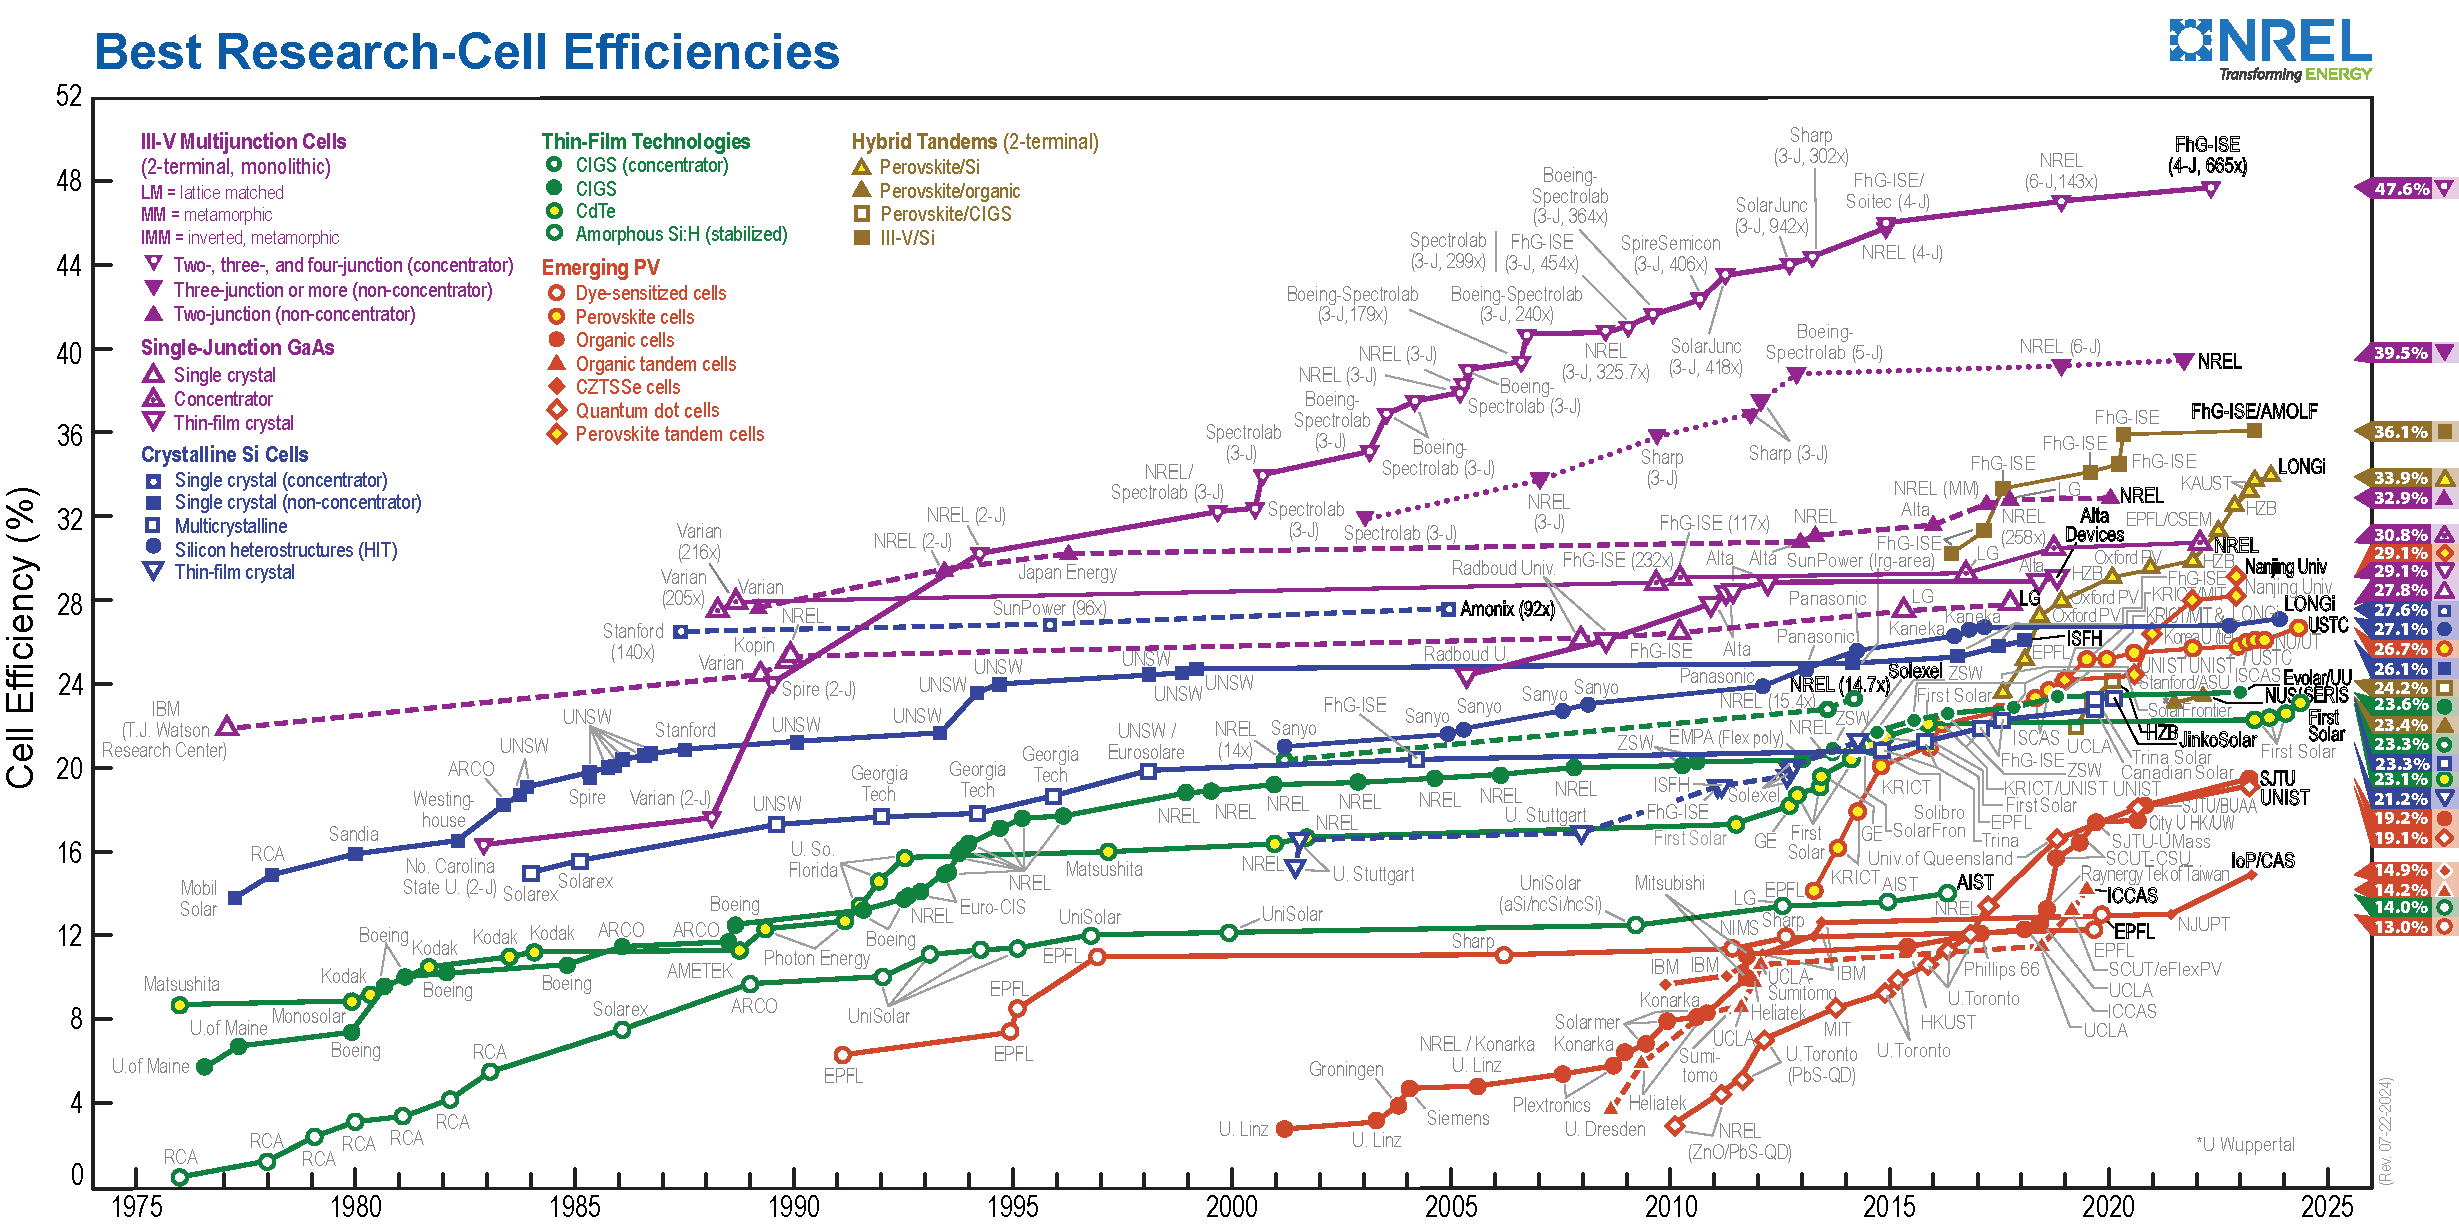
\includegraphics[keepaspectratio,width=0.8\textwidth,height=0.5\textheight]{figuras/cell-efficiencies.pdf}
\caption{\label{fig:orgc35b32b}Evolución de la eficiencia de células según la tecnología (según el National Renewable Energy Laboratory \cite{nrel24} (EEUU)).}
\end{figure}

\subsubsection{Influencia de la temperatura y la radiación}
\label{sec:org2800402}
La temperatura y la radiación son factores cruciales en el funcionamiento de una célula solar. El aumento de la temperatura ambiente reduce la tensión de circuito abierto según la relación \(dV_{oc}/dT_c\), \nomenclature[Tc]{\(T_c\)}{Temperatura de célula} que para células de silicio cristalino es de\(-2,3\frac{mV}{^\circ C}\). Además, disminuye la eficiencia de la célula solar con \(\frac{d\eta}{dT_c}=-0,4\%/^\circ C\).

En cuanto a la iluminación, la fotocorriente y la tensión de circuito abierto son proporcionales a la irradiancia incidente.

Tomando en cuenta estas influencias, se definen una condiciones de funcionamiento, denominadas condiciones estándar de medida (STC)\nomenclature[STC]{STC}{Condiciones estándar de medida de un dispositivo fotovoltaico}, válidas para caracterizar una célula en el entorno de un laboratorio. Estas condiciones vienen determinadas por:
\begin{itemize}
\item Irradiancia: \(G_{stc}=1000W/m^2\) con incidencia normal
\nomenclature[GSTC]{\(G_{STC}\)}{Irradiancia incidente en condiciones estandar de medida}
\item Temperatura de célula: \(T_c^*=25^\circ C\) \nomenclature[TC*]{\(T_c^*\)}{Temperatura de célula en condiciones estándar de medida}
\item Masa de aire: \(AM=1,5\)\footnote{Relación entre el camino recorrido por los rayos directos del Sol a través de la atmósfera hasta la superficie receptora y el que recorrerían en caso de incidencia vertical (\(AM=1/cos\theta_{zs}\)).}
\end{itemize}
Frecuentemente los fabricantes informan de los valores de las tensiones \(V_{oc}^*\) y \(V_{mpp}^*\) y las corrientes \(I_{sc}^*\) y \(I_{mpp}^*\)\footnote{Es de uso común añadir un asterisco como superíndice para denotar aquellos parámetros medidos en estas condiciones.}. A partir de estos valores es posible referir a estas condiciones:
\begin{itemize}
\item La potencia: \(P_{mpp}^*=I_{mpp}^*\cdot V_{mpp}^*\)
\item El factor de forma: \(FF^*=\frac{P_{mpp}^*}{I_{sc}^*\cdot V_{oc}^*}\)
\item La eficiencia: \(\eta^*=\frac{I_{mpp}^*\cdot V_{mpp}^*}{A_c\cdot G_{stc}}\)
\end{itemize}

\subsection{Funcionamiento de un módulo fotovoltaico}
\label{sec:org1675715}
\label{subsec:funcionamiento-modulo-fotovoltaico}
\subsubsection{Comportamiento térmico de un módulo}
\label{sec:orgb93d130}
La mayoría de las ecuaciones que definen el comportamiento de un módulo fotovoltaico\footnote{Los cálculos de este apartado, quedan recogidos en la función \texttt{fProd}.} se establecen en lo que se conoce como condiciones estándar de funcionamiento. En estas condiciones, la temperatura de la célula es de \(25^\circ C\). Sin embargo, la temperatura de operación de la célula es diferente y depende directamente de la radiación que recibe el módulo en cada momento.

El módulo recibe una cantidad de radiación dada, absorbiendo la fracción de esta que no se refleja al exterior. De dicha fracción, parte de ella es transformada en energía eléctrica, mientras que el resto se entrega en forma de calor al entorno.

Para simplificar, se puede asumir que el incremento de la temperatura de la célula respecto de la temperatura ambiente depende linealmente de la irradiancia incidente en esta. El coeficiente de proporcionalidad depende de muchos factores, tales como el modo de instalación del módulo, la velocidad del viento, la humedad ambiente y las características constructivas del laminado.

Estos factores quedan recogidos en un valor único representado por la temperatura de operación nominal de célula (NOCT o TONC)\nomenclature[TONC]{\(TONC\)}{Temperatura de operación nominal de célula}, definida como aquella que alcanza una \emph{célula} cuando su \emph{módulo} trabaja en las siguientes condiciones:
\begin{itemize}
\item Irradiancia: \(G=800W/m^2\)
\item Masa de aire: \(AM= 1,5\)
\item Irradiancia normal
\item Temperatura \emph{ambiente}: \(T_a=20^\circ C\)
\item Velocidad de viento: \(v_v=1m/s\)
\end{itemize}

La ecuación \ref{eq:temp-cel} expresa una aproximación aceptable del comportamiento térmico de una célula integrada en un módulo en base a las consideraciones previas:
\begin{equation}
T_c=T_a+G_{ef}\cdot \frac{NOCT-20}{800}
\label{eq:temp-cel}
\end{equation}
Para la simulación del funcionmaiento de un módulo fotovoltaico en condiciones de operación real, es necesario contar con secuencias de valores de temperatura ambiente. Si no se dispone de información detallada, se puede asumir un valor constante de \(T_a=25^\circ C\) para simulaciones anuales. Sin embargo, si se conocen los valores máximos y mínimos diarios de la temperatura ambiente, se puede generar una secuencia intradiaria usando una combinación de funciones coseno:
\begin{enumerate}
\item \textbf{Calcular los valores de} \(T_m\) \textbf{y} \(T_r\): Se definen los valores de la temperatura media diaria, \(T_m\) simplemente como la media entre la \(T_{max}\) y la \(T_{min}\):
\nomenclature[Tmax]{$T_{max}$}{Temperatura máxima en un día}
\nomenclature[Tmin]{$T_{min}$}{Temperatura mínima en un día}
\begin{equation}
T_m=\frac{T_{max}+T_{min}}{2}
\end{equation}
y la mitad de la amplitud de temperaturas, \(T_r\):
\begin{equation}
T_r=\frac{T_{max}-T_{min}}{2}
\end{equation}
\item \textbf{Calcular la matriz de} \(T_a\): Una vez obtenidos los valores de \(T_m\) y \(T_r\), el siguiente paso es calcular la matriz de valores de temperatura ambiental \(T_a\) para cada hora. Para ello, se deben calcular 3 valores auxiliares:
\nomenclature[Ta]{Ta}{Temperatura ambiente}
\begin{equation}
a_1=\frac{12\pi \cdot (\omega_s-\omega)}{21\pi+12\cdot \omega_s}
\end{equation}
\begin{equation}
a_2=\frac{\pi \cdot (3\pi -12\omega)}{3\pi - 12\omega}
\end{equation}
\begin{equation}
a_3=\frac{\pi (24\pi + 12 \cdot (\omega_s - \omega))}{21 \cdot \pi + 12 \cdot \omega_s}
\end{equation}
Con estos tres valores se pueden calcular la terna de temperaturas \(T_1\), \(T_2\), \(T_3\):
\begin{equation}
T_1 = T_m-T_r\cdot\cos(a_1)
\end{equation}
\begin{equation}
T_2 = T_m+T_r\cdot\cos(a_2)
\end{equation}
\begin{equation}
T_3=T_m-T_r\cdot\cos(a_3)
\end{equation}
\item \textbf{Selección del valor clave}: Se selecciona el valor adecuado de \(T_a\) en base al siguiente criterio:
\begin{equation}
T_a = \begin{cases}
T_1& \text{si $\omega \leq \omega_s$}\\
T_2& \text{si $\omega_s < \omega \leq \frac{\pi}{4}$}\\
T_3& \text{si $\omega > \frac{\pi}{4}$}
\end{cases}
\end{equation}
\end{enumerate}
\subsubsection{Cálculo de \(V_{oc}\) y \(I_{sc}\)}
\label{sec:orgb41c583}
Conocidos los valores horarios de temperatura de la célula, se puede calcular \(V_{oc}\) utilizando la ecuación \ref{eq:ten-ca}. Y, por último, mediante la ecuación \ref{eq:int-cc} se puede calcular \(I_{sc}\).
\begin{equation}
V_{oc}(T_c)=V_{oc}^*+(T_c-T_c^*)\cdot \frac{dV_{oc}}{dT_c}\cdot N_{cs}
\label{eq:ten-ca}
\end{equation}
\begin{equation}
I_{sc}=G_{ef}\cdot \frac{I_{sc}^*}{G^*}
\label{eq:int-cc}
\end{equation}

\subsubsection{Factor de forma variable}
\label{sec:orgea7dd31}
Una vez obtenidos los valores de \(V_{oc}\) y \(I_{sc}\), el siguiente paso ha de ser calcular los valores de tensión y corriente en el punto de máxima potencia, pues es donde el generador estará entregando su máxima potencia, como su propio nombre indica. Por tanto, es un punto de interés para el cálculo.

Existen dos metodologías de cálculo de dicho punto, uno de ellos significantemente más sencillo que el otro. Este consiste en suponer que el Factor de Forma, definido en la expresión \ref{eq:factor-forma}, es constante.

Si suponemos que FF es constante, se podrían extraer los valores de tensión y corriente en el punto de máxima potencia, ya que si
\begin{equation}
FF=FF^*
\end{equation}
entonces
\begin{equation}
\frac{I_{mpp}\cdot V_{vmpp}}{I_{sc}\cdot V_{oc}}=\frac{I_{mpp}^*\cdot V_{vmpp}^*}{I_{sc}^*\cdot V_{oc}^*}
\end{equation}
pudiendo así obtener los valores de \(I_{mpp}\) y \(V_{vmmp}\).

Sin embargo, este suposición da resultados alejados a una estimación acertada. Por ello, se tendrá en cuenta la variación del factor de forma:
\begin{itemize}
\item \textbf{Cálculo de la tensión termica, \(V_t\), a temperatura de la célula}: se calculará el valor de \(V_t\) a 25ºC con la expresión:
\begin{equation}
V_{tn}=\frac{V_t\cdot (273+25)}{300}
\end{equation}
\item \textbf{Cálculo de \(R_s^*\)}: el segundo paso consiste en calcular el valor de resistencia en serie con los valores STC:
\begin{equation}
R_s^*=\frac{\frac{V_{oc}^*}{N_{cs}}-\frac{V_{mpp}^*}{N_{cs}}+m\cdot V_{tn}\cdot ln(1-\frac{I_{mpp}^*}{I_{sc}^*})}{\frac{I_{mpp}^*}{N_{cp}}}
\end{equation}
\item \textbf{Cálculo de \(r_s\)}: utilizando el valors de \(R_s^*\), calculado en el paso anterior junto con los valores de \(V_{oc}\) y \(I_{sc}\), podemos calcular \(r_s\) que se utilizará más adelante en el proceso.
\begin{equation}
r_s=R_s^*\cdot (\frac{N_{cs}}{N_{cp}}\cdot \frac{I_{sc}}{V_{oc}})
\end{equation}
\item \textbf{Cálculo de \(k_{oc}\)}: a continuación, utilizando los valores de temperatura ambiente obtenidos con anterioridad junto con la tensión de circuito abierto, se calcula \(k_{oc}\) mediante la expresión:
\begin{equation}
k_{oc}=\frac{V_{oc}/N_{cs}}{m\cdot V_t \cdot \frac{T_c+273}{300}}
\end{equation}
\end{itemize}

Con los cálculos previos, este método propone localizar el punto de máxima potencia de forma aproximada mediante las ecuaciones:
\begin{equation}
i_{mpp}=1-\frac{D_M}{k_{oc}}
\end{equation}
\begin{equation}
v_{mpp}=1-\frac{ln(k_{oc}/D_M)}{k_{oc}}-r_s\cdot i_{mpp}
\end{equation}
donde:
\begin{equation}
D_M=D_{M0}+2\cdot r_s\cdot D_{M0}^2
\end{equation}
\begin{equation}
D_{M0}=\frac{k_{oc}-1}{k_{oc}-lnk_{oc}}
\end{equation}

Por último, multiplicando los valores de \(i_{mpp}\) y \(v_{mpp}\) por \(I_{sc}\) y \(V_{oc}\) respectivamente, se obtienen los valores de \(I_{mpp}\) y \(V_{mpp}\), que serán los que se utilicen para calcular la potencia entregada por el generador en el punto de máxima potencia.

Teniendo estos valores se puede obtener:
\begin{equation}
P_{mpp}=I_{mpp}\cdot V_{mpp}
\end{equation}

\subsection{Cálculo de potencias y energías de un sistema fotovoltaico conectado a la red}
\label{sec:orgbeacf32}
\label{subsec:calculo-potencias-energias}
La potencia obtenida en el paso anterior es la de un solo módulo. Para conocer la potencia que va a ser capaz de entregar un SFCR, se debe tener en cuenta su configuración de módulos en serie y en paralelo\footnote{Los cálculos de este apartado, quedan recogidos en las funciones \texttt{fProd} y \texttt{prodCGPV}.}.
\begin{equation}
P_g^*=N_s\cdot N_p\cdot P_m^*
\end{equation}
Con este paso se obtiene la potencia horaria entregada por el generador fotovoltaico. El siguiente paso será pasar esa potencia a través del inversor y calcular la potencia a la salida de este.

Primero, se esteblecen las expresiones de las potencias normalizadas, siendo \(P_{inv}\) la potencia nominal del inversor:
\nomenclature[Pinv]{\(P_{inv}\)}{Potencia nominal de un inversor}
\begin{equation}
p_i=\frac{P_{DC}}{P_{inv}}
\end{equation}
\begin{equation}
p_o=\frac{P_{AC}}{P_{inv}}
\end{equation}

Por otro lado, el rendimiento de un inversor fotovoltaico se puede modelizar de la siguiente manera:
\begin{equation}
\eta_{inv}=\frac{p_o}{p_o+k_0+k_1p_o+k_2p_o^2}
\end{equation}

De las dos ecuaciones anteriores se puede deducir:
\begin{equation}
p_i=p_o+k_0+k_1p_o+k_2p_o^2
\end{equation}

Desarrollando esta ecuación, se puede obtener una ecuación de segundo grado con \(p_o\) como incógnita:
\begin{equation}
k_2p_o^2+(k_1+1)p_o+(k_0-p_i)=0
\end{equation}

Por último, volviendo a las primeras expresiones, se puede obtener la potencia en corriente alterna:
\begin{equation}
P_{AC}=p_o\cdot P_{inv}
\end{equation}

Con esta potencia, integrando en función del tiempo, se puede obtener la energía que genera el sistema
\begin{equation}
E_{AC}=\int_{T} P_{AC} \,dt
\end{equation}
y la productividad:
\begin{equation}
Y_f=\frac{E_{ac}}{P_g^*}
\end{equation}

\subsection{Cálculo de potencias y energías de un sistema fovoltaico de bombeo}
\label{sec:orge4ff597}
\subsubsection{Potencia hidráulica}
\label{sec:org93b5939}
La potencia hidráulica, \(P_H\) \nomenclature[PH]{$P_H$}{Potencia hidráulica}, necesaria para bombear agua es función de:
\begin{itemize}
\item La altura vertical aparente, \(H_v\) \nomenclature[Hv]{$H_v$}{Altura vertical aparente}
\item El caudal de agua, \(Q\) \nomenclature[Q]{$Q$}{Caudal de agua} \nomenclature[g]{$g$}{Aceleración de la gravedad} \nomenclature[rho]{$\rho$}{Densidad del agua}
\end{itemize}
\begin{equation}
P_H=g\cdot \rho \cdot Q \cdot H_V
\end{equation}

Expresando \(P_H\) en watios, \(H_v\) en metros y \(Q\) en \(m^3/h\) la ecuación resulta en:
\begin{equation}
P_H=2.725\cdot Q \cdot H_v
\end{equation}

Asumiendo que el agua bombeado sale por el coducto a baja velocidad, la potencia de salida de la bomba necesita satisfacer \(P_H\) \nomenclature[PH]{$P_H$}{Potencia hidraúlica necesaria en un sistema de bombeo de agua}, más las pérdidas de fricción en la tubería, \(P_f\) \nomenclature[Pf]{$P_f$}{Pérdidas de frición en la tubería de un sistema de bombeo}. Este valor se asimila a una altura equivalente \(H_f\), \nomenclature[Hf]{$H_f$}{Altura asociada a las pérdidas de frición en una tubería} asociado a un caudal determinado: \nomenclature[HT]{$H_T$}{Altura total incluyendo las pérdidas de fricción de la tubería}
\begin{equation}
H_T=H_v+H_f
\end{equation}
La potencia eléctrica a la entrada de la motobomba, \(P_{el}\), es:
\nomenclature[Pel]{$P_{el}$}{Potencia eléctrica necesaria en la entrada de una motobomba}
\begin{equation}
P_{el}=\frac{P_H+P_f}{\eta_{mp}} 
\end{equation}
donde \(\eta_{mp}\) es la eficiencia de la motobomba.
\nomenclature[etamp]{$\eta_{mp}$}{Eficiencia de una motobomba}
La potencia eléctrica requerida por la motobomba es entregada por un generador FV y acondicionador de potencia:
\begin{equation}
P_{el}=P_g^* \cdot \frac{G}{G_{stc}} \frac{\eta_g}{\eta_g^*} \cdot \eta_{inv}
\end{equation}
siendo \(G\) la irradiancia en el plano del generador, \(eta_{inv}\) la eficiencia del equipo de acondicionamiento de potencia y \(\frac{\eta_g}{\eta_g^*}\) modela el comportamiento del generador con la temperatura.

\subsubsection{Caudal diario}
\label{sec:org19776f0}
El caudal diario bombeado por este conjunto es:
\begin{equation}
Q_d = \int_{d} \frac{G}{G^*} \cdot P_g^* \cdot \eta_g \cdot \frac{\eta_{ig}}{\eta_{ig}^*} \cdot \eta_{inv} \cdot \eta_{mp} \, dt
\end{equation}

\subsubsection{Altura}
\label{sec:org56613b0}
Se puede definir una altura total equivalente, \(H_{TE}\), con las siguientes suposiciones:
\nomenclature[HTE]{$H_{TE}$}{Altura total equivalente de un sistema de bombeo}
\begin{itemize}
\item Las pérdidas de fricción en tubería son despreciables (\(H_f < 0.05 \cdot H_T\)).
\item El nivel del agua dentro del pozo se mantiene constante.
\end{itemize}
\begin{equation}
Q_d = \frac{P^*_g}{2.725 \cdot G^* \cdot H_{TE}} \int \left( \frac{G}{\eta_{ig}^{*} \eta_{m}^{*} \eta_{inv} \eta_{mp}} \right) dt
\end{equation}
Ahora el cálculo en la integral solo depende de la radiación, temperatura, y equipos.

Para calcular esta altura total equivalente, se debe suponer que:
\begin{itemize}
\item El pozo está caracterizado con tres parámetros:
\begin{itemize}
\item Nivel estático, \(H_{st}\)
\nomenclature[Hst]{$H_{st}$}{Nivel estático de un pozo}
\item Nivel dinámico, \(H_{dt}\)
\nomenclature[Hdt]{$H_{dt}$}{Nivel dinámico de un pozo}
\item Caudal de ensayo, \(Q_t\) \nomenclature[Qt]{$Q_t$}{Caudal de ensayo de un pozo}
\end{itemize}
\item Que se ha realizado el ensayo de bombeo para caracterizar los pozos con bomba portátil empleando el caudal máximo del pozo, \(Q_{max}\) (\(Q_t=Q_{max}\)).
\nomenclature[Qman]{$Q_{max}$}{Caudal máximo del pozo}
\end{itemize}

Con estas suposiciones se puede llegar a la expresión:
\begin{equation}
H_{TE} = H_{ot} + H_{st} + \left( \frac{H_{dt} - H_{st}}{Q_T} \right) Q_{AP} + H_f(Q_{AP})
\end{equation}
donde:
\begin{itemize}
\item \(H_{OT}\), es la altura desde la salida de agua hasta el suelo.
\nomenclature[HOT]{$H_{OT}$}{Diferencia de cotas entre la salida de agua y la entrada en el depósito}
\item Nivel estático, \(H_{st}\).
\item Nivel dinámico, \(H_{dt}\).
\item Caudal aparente, \(Q_{AP} = \alpha \cdot Q_d\)
(\(\alpha=1/24=0.0416h^{-1}\)).
\item \(H_f(Q_{AP})\), pérdidas en la tubería al caudal aparente.
\end{itemize}

\subsubsection{Potencia del generador}
\label{sec:orga22ff8c}
Como primera aproximación, se consideran constantes a lo largo del tiempo las eficiencias de los componentes del sistema con la elección de ciertos valores adecuados (\(\frac{\eta_g}{\eta_g^*}=0.85, \eta_{mp}=0.35, \eta_{inv}=0.9\)). Así, es posible calcular de forma aproximada la potencia nominal del generador necesaria para bombear un caudal diario \(Q_d\) a una altura total equivalente \(H_{TE}\) a partir de la ecuación:
\begin{equation}
P^*_g = \frac{10 \cdot HTE \cdot Q_d}{\frac{G_d}{G_{stc}}}
\end{equation}

\subsubsection{Simulación de sistemas fotovoltaicos de bombeo}
\label{sec:org9d470d1}
Debido a la complicación del cálculo del dimensionamiento de los sistemas fotovoltaicos de bombeo, se puede recurrir a métodos de simulación asistidos por ordenador\footnote{Correspondientes a la función \texttt{fPump}.}. El algoritmo a seguir es:
\begin{enumerate}
\item Curva característica de la bomba que relaciona la altura, \(H\), y el caudal, \(Q\), a la frecuencia nominal de la bomba:
\begin{equation}
H = a \cdot f^2 + b \cdot f \cdot Q + c \cdot Q^2
\end{equation}
\begin{itemize}
\item Donde \(a\), \(b\), y \(c\) son coeficientes característicos de la bomba y \(f\) es la frecuencia.
\end{itemize}
\item Relaciones de semejanza para bombas centrífugas:
\begin{equation}
\frac{f_1}{f_2} = \frac{Q_1}{Q_2} = \left(\frac{H_1}{H_2}\right)^{1/2} = \left(\frac{P_1}{P_2}\right)^{1/3}
\end{equation}
\item Cálculo de caudal y altura a frecuencia nominal (50 Hz):
\begin{equation}
Q_{50} = \frac{50 \cdot Q}{f}
\end{equation}
\begin{equation}
H_{50} = H \cdot \left(\frac{50}{f}\right)^2
\end{equation}
\item Ecuación de potencia hidráulica:
\begin{equation}
P_{h,50} = 2.725 \cdot Q_{50} \cdot H_{50}
\end{equation}
\item Potencia mecánica en el eje de la bomba a 50 Hz:
\begin{equation}
P_{b,50} = \frac{P_{h,50}}{\eta_b}
\end{equation}
\item Potencia mecánica a frecuencia \(f\):
\begin{equation}
P_b = P_{b,50} \cdot \left(\frac{f}{50}\right)^3
\end{equation}
\item Potencia eléctrica demandada por el motor:
\begin{equation}
P_{bc} = P_b \cdot \frac{50}{f}
\end{equation}
\begin{equation}
P_{e,50} = \frac{P_{bc}}{\eta_m}
\end{equation}
\begin{equation}
P_e = P_{e,50} \cdot \frac{f}{50}
\end{equation}
\item Perfil de irradiancia diaria (según IEC 61725):
\begin{equation}
G = G_{max} \cdot \cos\left(\frac{t}{t_0} \cdot \frac{\pi}{2}\right) \cdot \left[1 + s \cdot \left(1 - \cos\left(\frac{t}{t_0} \cdot \frac{\pi}{2}\right)\right)\right]
\end{equation}
donde G es la irradiancia (\(W/m^2\)) en la hora \(t\), \(G_{max}\) es el valor máximo de irradiancia (\(W/m^2\)) durante el día en cuestión y \(s\) es el factor de forma definido por:
\begin{equation}
s = \frac{d \cdot \frac{\pi}{2} - 1}{1 - \frac{\pi}{4}}
\end{equation}
siendo \(d\) el factor de conjunto de datos calculado con:
\begin{equation}
d = \frac{G_d}{G_{max} \cdot h}
\end{equation}
\end{enumerate}

\section{Sombras y ocupación de terreno}
\label{sec:org920954c}
Al diseñar una central fotovoltaica se debe decidir la ubicación de las diferentes partes del generador resolviendo un compromiso entre la mejor ocupación del terreno disponible y la minimización del impacto de sombras mutuas arrojadas entre los módulos\footnote{Correpondiente a las funciones \texttt{calcShd} (cálculo de sombras) y \texttt{optimShd} (optimización de distancias).}.

Este factor de sombras implica un nivel de ocupación de terreno que depende del modo de seguimiento del generador. La ocupación del terreno se puede medir con dos métricas:
\begin{itemize}
\item \textbf{Relación de ocupación del terreno} (\emph{Ground Coverage Ratio}, \(GCR\)): es la relación entre el área del generador, \(A_G\), y el área del terreno ocupado, \(A_T\) (por tanto, siempre será GCR < 1). \nomenclature[AG]{$A_G$}{Área de un generador fotovoltáico} \nomenclature[GCR]{$GCR$}{Ground coverage ratio}
\begin{equation}
GCR = \frac{A_G}{A_T}
\end{equation}
\item \textbf{Ratio de ocupación del terreno} (\(ROT\), o \emph{Ground Requirement Ratio}, \(GRR\)): es el inverso del GCR, la relación entre el área de terreno ocupado, \(A_T\), y el área del generador, \(A_G\). \nomenclature[ROT]{$ROT$}{Ratio de ocupación del terreno}
\begin{equation}
ROT = \frac{A_T}{A_G}
\end{equation}
\end{itemize}

\subsection{Sistemas estáticos}
\label{sec:org079b013}
Las filas que componen el generador arrojan sombras unas sobre otras en determinados momentos del días y año. Como recomendación general, es de uso común respetar un mínimo de 4 horas de sol en torno al mediodía del solsticio de invierno libres de sombra. La longitud de la sombra de un obstáculo se mide con:
\begin{equation}
d = \frac{h}{tan\gamma_s}
\end{equation}
siendo \(h\) la altura de la fila adyacente, \(h=L\cdot sin(\beta)\), y \(L\) la longitud del generador, según se indica en la figura \ref{fig:sombras-estaticos}.
\begin{figure}[htbp]
\centering
\includegraphics[width=.9\linewidth]{figuras/SombrasEstaticas.pdf}
\caption{Dimensiones y distancias entre filas de un sistema estático. Figura 6.10 del libro ESF \cite{Perpinan2023}. \label{fig:sombras-estaticos}}
\end{figure}

En el mediodía del solsticio de invierno, la altura solar es \(\gamma_s = 90^\circ - 23.45^\circ - |\phi| \simeq 67^\circ - |\phi|\). Por tanto, la distancia mínima que permite 4 horas libres de sombra alrededor del mediodía es:
\nomenclature[dmin]{$d_{min}$}{Distancia mínima entre hileras de un generador para evitar el sombreado}
\begin{equation}
d_{min}=\frac{h}{tan(61^\circ - |\phi|)}
\end{equation}

\subsection{Sistemas de seguimiento a doble eje}
\label{sec:org65be50d}
El diseño de un sistema de seguimiento solar a doble eje busca optimizar la ubicación de los seguidores para minimizar las pérdidas de radiciación por sombras, utilizando eficientemente el terreno. Para esto, se simula el sistema en diferentes configuraciones y se elige la más eficiente en términos de productividad y ROT, que se calcucula con la fórmula:
\begin{equation}
ROT = \frac{L_{ns}\cdot L_{eo}}{L\cdot W}
\end{equation}
donde (figuras \ref{fig:sombras-doble} y \ref{fig:dimensiones-sombras-doble}):
\begin{itemize}
\item \(L_{ns}\) es la separación entre seguidores en la dirección Norte-Sur.
\nomenclature[Lns]{$L_{ns}$}{Separación entre seguidores en sentido Norte-Sur}
\item \(L_{eo}\) es la separación en la dirección Este-Oeste.
\nomenclature[Leo]{$L_{eo}$}{Separación entre seguidores en sentido Este-Oeste}
\item \(L\) es la longitud del seguidor.
\item \(W\) es la anchura del seguidor.
\end{itemize}

\begin{figure}[htbp]
\centering
\includegraphics[height=0.2\textheight]{figuras/Sombras2X.pdf}
\caption{Sombras mutuas en un conjunto de cuatro seguidores. Figura 6.11 del libro ESF \cite{Perpinan2023}. \label{fig:sombras-doble}}
\end{figure}
\begin{figure}[htbp]
\centering
\includegraphics[height=0.2\textheight]{figuras/DimensionesSeguidorSombra.pdf}
\caption{Dimensiones de un seguidor a doble eje y longitud de su sombra arrojada. Figura 6.12 del libro ESF \cite{Perpinan2023}. \label{fig:dimensiones-sombras-doble}}
\end{figure}
\begin{figure}[htbp]
\centering
\includegraphics[height=0.2\textheight]{figuras/SixTrackerShadow.pdf}
\caption{Posibles sombras en un conjunto de seis seguidores. Figura 6.13 del libro ESF \cite{Perpinan2023}. \label{fig:conjunto-seis-seguidores}}
\end{figure}


El sistema se modela como un grupo de seis seguidores en una matriz de dos filas en dirección Norte-Sur (figura \ref{fig:conjunto-seis-seguidores}), representando tres situaciones de sombra: lateral (Este-Oeste), frontal (Norte-Sur) y diagonal, caracterizados por los factores de sombra \(FS_{xx}\) (definidos como la relación entre el área sombreada y el área total del generador). Las ecuaciones para estos factores son, en las que se emplean los valores normalizados de las distancias, \(l_{eo}=\frac{L_{eo}}{W}\) y \(l_{ns}=\frac{L_{ns}}{W}\):
\begin{equation}
\begin{array}{c}
|l_{eo}\cdot\cos(\psi_{s})|<1\\
|l_{eo}\cdot\sin(\psi_{s})|<s\end
{array}
\Rightarrow
FS_{eo}=\frac{(1-|l_{eo}\cos(\psi_{s})|)\cdot(s-|l_{eo}\sin(\psi_{s})|)}{s}
\end{equation}
\begin{equation}
\begin{array}{c}
|l_{ns}\cdot\cos(\psi_{s})|<s\\
|l_{ns}\cdot\sin(\psi_{s})|<1
\end{array}
\Rightarrow 
FS_{ns}=\frac{(s-|l_{ns}\cos(\psi_{s})|)\cdot(1-|l_{ns}\sin(\psi_{s})|)}{s}
\end{equation}
\begin{align*}
\begin{array}{c}
s>|l_{ns}\cdot\cos(\psi_{s})|+|l_{eo}\sin(\psi_{s})|\\
1>|l_{eo}\cdot\cos(\psi_{s})|-|l_{ns}\cdot\sin(\psi_{s})|
\end{array} 
& \Rightarrow
\end{align*}
\begin{equation}
FS_{d}=\frac{\left[s-\left(|l_{eo}\cdot\sin(\psi_{s})|+|l_{ns}\cos(\psi_{s})|\right)\right]\cdot\left[1-\left(|l_{eo}\cdot\cos(\psi_{s})|-|l_{ns}\sin(\psi_{s})|\right)\right]}{s}
\end{equation}
siendo \(\psi_{s}\) el acimut solar y \(\gamma_{s}\) la altura solar y donde la longitud de sombra (normalizada con la anchura del seguidor) se calcula con:
\begin{align}
s & =s_{1}+s_{2}\\
s_{1} & =b\cdot\cos(\beta)\\
s_{2} & =\frac{b\cdot\sin(\beta)}{\vert\tan(\gamma_{s})\vert}
\end{align}
El factor \(\frac{\sin(\gamma_{s})}{\sin(\gamma_{s}+\beta)}\) representa 
la proyección de sombra existente en el suelo sobre el plano del generador, y por tanto, el porcentaje de área sombreada que debe ser eliminado de la radiación directa. Desarrollando este factor, se obtiene una formulación alternativa que puede facilitar el cálculo de los tres factores:
\begin{align}
FS_{eo} & =\frac{(1-l_{eo}\cos(\psi_{s}))\cdot(s-l_{eo}\sin(\psi_{s}))}{s}\\
FS_{ns} & =\frac{(s-l_{ns}\cos(\psi_{s}))\cdot(1-l_{ns}\sin(\psi_{s}))}{s}\\
FS_{d} & =\frac{\left[s-\left(l_{eo}\cdot\sin(\psi_{s})+l_{ns}\cos(\psi_{s})\right)\right]\cdot\left[1-\left(l_{eo}\cdot\cos(\psi_{s})-l_{ns}\sin(\psi_{s})\right)\right]}{s}
\end{align}

Realizando la simulación de este sistema, incluyendo el cálculo de sombras y repitiendo la simulación para varias combinaciones (Lns, Leo) pueden elaborarse gráficos de nivel como el de la figura \ref{fig:abaco-sombras}. En estas, se recoge el ratio entre la energía anual producida por un seguidor \emph{promedio} incluyendo el efecto de por sombras mutuas\footnote{En el cálculo de la producción del seguidor afectado por sombras mutuas, se considera que la reducción en potencia está exclusivamente relacionada con el área sombreada, por tanto, no se tienen en cuenta las conexiones eléctricas entre módulos.} y la energía anual producida por un seguidor sin sombreado.
\begin{figure}[htbp]
\centering
\includegraphics[height=0.4\textheight]{figuras/AbacoSombras.pdf}
\caption{Ábaco para planta de seguimiento a doble eje. Recoge el ratio entre la energía anual producida por un seguidor afectado por sombras mutuas (\(E_{acS}\)) y la producida por un seguidor sin sombreado (\(E_{ac0}\)). Las curvas de color negro representan la fracción de energía no afectada por sombras. Las curvas de puntos representan el valor del ROT. Figura 6.14 del libro ESF \cite{Perpinan2023}. \label{fig:abaco-sombras}}
\end{figure}

\subsection{Sistemas de seguimiento de eje horizontal}
\label{sec:org66dc20e}
Se considera que los seguidores son de longitud infinita en sentido Norte-Sur (se desprecia el efecto de borde). Así, los parámetros que determinan el diseño de este tipo de sistema son (figura \ref{fig:SeguidorEjeHorizontalSombras}):
\begin{figure}[htbp]
\centering
\includegraphics[scale=0.9]{figuras/SombrasHoriz.pdf}
\caption{Dimensiones básicas en sistemas con seguidores de eje horizontal. Figura 6.16 del libro ESF \cite{Perpinan2023}. \label{fig:SeguidorEjeHorizontalSombras}}
\end{figure}
\begin{enumerate}
\item La inclinación del generador fotovoltaico, \(\beta\), (coincidente con el ángulo \(\psi_{ns}\)).
\item La dimensión en sentido Este-Oeste del campo generador, L.
\item La separación entre los diferente seguidores en la dirección Este-Oeste, \(L_{eo}\).
Por tanto, \(ROT=\frac{L_{eo}}{L}\).
\end{enumerate}

Para caracterizar numéricamente el sombreado, se empreará el factor \(FS_{eo}\). Mediante consideraciones geométricas, utilizando la distancia normalizada \(l_{eo}=\frac{L_{eo}}{L}\), es posible escribir:
\begin{align}
FS_{eo} & =\frac{s-l_{eo}}{s}\nonumber \\
 & =1-l_{eo}\cdot\cos(\beta)\nonumber \\
 &
 =1-l_{eo}\cdot\frac{\sin(\omega)}{\sqrt{\sin^{2}(\omega)+\left(\cos(\omega)\cos(\phi)+\tan(\delta)\sin(\phi)\right)^{2}}}\label{eq:FSeoHorizontal}
\end{align}

\subsubsection{Limitación de ángulo y retroseguimeitno}
\label{sec:org76fdb77}
En seguidores de eje horizontal se puede evitar la incidencia de sombras en cualquier en cualquier instante mediante algoritmos de \emph{backtracking} o retroseguimiento \cite{Panico.Garvison.ea1991}. Esta técnia provoca el desvío del seguidor de su posición óptima en los instantes en los que se produce la sombra entre seguidores, evitando el impacto de sombras pero con la consiguiente reducción en energía producida pro alejamiento del apuntamiento óptimo.

Para evitar la aparición de sombras, el ángulo de inclinación de los seguidores debe ser tal que la longitud de la sombra sea igual a la distancia entre seguidores. Siendo \(\beta\) el ángulo de inclinación con retroseguimiento, y \(\beta_0\) el ángulo de inclinación original. De la ecuación \ref{eq:FSeoHorizontal} se deduce que sólo será necesario aplicar esta técnica cuando \(l_{eo}\cdot cos(\beta_0) \leq 1\). El triángulo definido por el rayo solar, el seguidor y la sombra debe cumplir la siguiente condición, basada en el teorema de los senos:
\begin{equation}
\label{eq:BT_senos}
\frac{l_{eo}}{\cos(\beta_0-\beta)}=\frac{1}{\cos{\beta_0}}
\end{equation}

Por tanto, el ángulo de inclinación que garantiza la ausencia de sombras a costa de apartarse de la condición de seguimiento es:
\begin{equation}
\label{eq:retroseguimiento}
\beta=\beta_0-\arccos(l_{eo}\cdot\cos{\beta_0})  
\end{equation}
ecuación que debe aplicarse solo cuando \(l_{eo} \cdot \cos(\beta_0) \leq 1\). En caso contrario, \(\beta = \beta_0\).
